\documentclass{beamer}

\usepackage{graphicx}
\usepackage{multicol}

\newcommand{\dif}{\ensuremath{\operatorname{d}\!}}

\usetheme{CambridgeUS}

\title[Prime Strings]{Prime Numbers Containing a Given String of Digits}
\subtitle{An Application of the Prime Number Theorem}
\author{Dylan Nelson}
\institute[SUMS]{Stellenbosch University Mathematics Society}
\date{8 April 2021}

\AtBeginSection[]{
    \begin{frame}
        \frametitle{Outline}
        \tableofcontents[currentsection]
    \end{frame}
}

\begin{document}

\frame{\titlepage}

\section{Background}

\begin{frame}
    \frametitle{Reddit Post}

    \begin{itemize}
        \item On 4 April 2016, a \href{https://www.reddit.com/r/math/comments/4d879s/most_surprising_divergent_series/}{thread was posted to /r/math on reddit} asking for the most surprising examples of divergent series.
        \begin{figure}
            \centering
            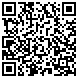
\includegraphics[width=0.25\textwidth]{reddit_thread.png}
            \caption{\url{https://www.reddit.com/r/math/comments/4d879s/most_surprising_divergent_series/}}
        \end{figure}
    \end{itemize}

\end{frame}

\begin{frame}
    \frametitle{Reddit Post — Primes with a Prime Number of Digits}

    \begin{itemize}
        \item In one example, we consider the set of prime numbers with a prime number of digits. \pause
        \item It is claimed that the sum of the reciprocals of the elements in this set diverges.
    \end{itemize}

    \begin{figure}
        \centering
        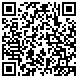
\includegraphics[width=0.25\textwidth]{reddit_prime_number_of_digits.png}
        \caption{\url{https://www.reddit.com/r/math/comments/4d879s/most_surprising_divergent_series/d1oppgu}}
    \end{figure}

\end{frame}

\begin{frame}
    \frametitle{Reddit Post — Numbers Without a $9$}

    \begin{itemize}
        \item In another example, we consider all of the positive integers that \emph{do not} have a $9$ \emph{anywhere} in their decimal expansion. \pause
        \item In this case, it is claimed that the sum of the reciprocals of these numbers \emph{converges}!
    \end{itemize}

    \begin{figure}
        \centering
        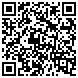
\includegraphics[width=0.25\textwidth]{reddit_kempner.png}
        \caption{\url{https://www.reddit.com/r/math/comments/4d879s/most_surprising_divergent_series/d1olh0o}}
    \end{figure}

\end{frame}

\begin{frame}
    \frametitle{Combining these Results}

    \begin{itemize}
        \item I realised that a combination of (appropriate generalisations) of these two claims implies that there are infinitely many primes which have a prime number of digits, and which contain any given string of decimal digits that you like. \pause
        \item And of course I promptly told everyone I know. \pause
        \item I even wrote a blog post about it!
        \begin{figure}
            \centering
            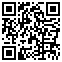
\includegraphics[width=0.25\textwidth]{mathemafrica_link.png}
            \caption{\url{http://www.mathemafrica.org/?p=12942}}
        \end{figure}
    \end{itemize}

\end{frame}

\begin{frame}
    \frametitle{This Talk}

    \begin{itemize}
        \item In this talk, we will prove this result following the argument presented in the blog post. \pause
        \item \emph{BUT}... by considering convergent and divergent series, the blog post is needlessly circuitous. \pause
        \item It is possible to give a more direct proof of a stronger result:
        \begin{block}{Proposition}
            Given a string of digits $S$, there is some natural number $N$, such that for all $n > N$, there is a prime with $n$ digits that starts with $S$. (Or by some non-zero digit followed by $S$.)
        \end{block} \pause
        \item I will present a proof of this more general proposition towards the end of the talk.
    \end{itemize}

\end{frame}

\section{The Harmonic and the Kempner Series}
\subsection{The Harmonic Series Diverges}

\begin{frame}
    \frametitle{The Harmonic Series}

    \begin{itemize}
        \item One of the first somewhat surprising examples of a divergent series that students are shown is the \emph{Harmonic Series}
        \[
            \sum_{n = 1}^{\infty} \frac{1}{n}.
        \]
        \item To show that this diverges, we group the terms in blocks of sizes equal to powers of $2$, and then approximate each term by the smallest element in its block.
        \begin{align*}
            \sum_{n = 1}^{\infty} \frac{1}{n} & = 1 + \sum_{n = 0}^{\infty} \sum_{k = 2^n + 1}^{2^{n + 1}} \frac{1}{k} \geq 1 + \sum_{n = 0}^\infty \sum_{k = 2^n + 1}^{2^{n + 1}} \frac{1}{2^{n + 1}} \\
            & = 1 + \sum_{n = 0}^{\infty} \frac{2^n}{2^{n + 1}} = 1 + \sum_{n = 0}^{\infty} \frac{1}{2}.
        \end{align*}
    \end{itemize}

\end{frame}

\begin{frame}
    \frametitle{The Harmonic Series}

    \begin{itemize}
        \item We of course get different behaviour if we sum the reciprocals of some subset of the natural numbers. \pause
        \item The sum of the reciprocals of the powers of $2$ converges:
        \[
            \sum_{n = 0}^{\infty} \frac{1}{2^n} = 2.
        \]
        \pause
        \item The sum of the reciprocals of the prime numbers diverges. \pause
        \item If we consider only the numbers that do not have a $9$ in their decimal expansion, the sum of the reciprocals of these numbers \emph{converges}. \pause
        \item This feels surprising because it seems like there should be relatively few primes and many, many numbers without a $9$ in their decimal expansion, but exactly the opposite is true.
    \end{itemize}

\end{frame}

\subsection{Reciprocals of Numbers Without a Given String of Digits}

\begin{frame}
    \frametitle{Reciprocals of Numbers Without a Given String of Digits}

    \begin{itemize}
        \item Let $S$ be any string of digits. Let $\mathbb{N}_S$ be the set of natural numbers that contain $S$ (contiguously) somewhere in their digits. \pause
        \item We will show that
        \[
            \sum_{n \not\in \mathbb{N}_S} \frac{1}{n}
        \]
        converges. \pause
        \item The approach will be similar to showing that the harmonic series diverges: we will group the digits in blocks of powers of $10^{\text{length of } S}$ and approximate the summands in each block by the largest element in the block.
    \end{itemize}

\end{frame}

\begin{frame}
    \frametitle{Reciprocals of Numbers Without a Given String of Digits}

    \begin{itemize}
        \item Let $m$ be the length of $S$. We group together the numbers with between $km + 1$ and $(k + 1)m$ digits for some $k \geq 0$.
        \[
            \sum_{n \not\in \mathbb{N}_S} \frac{1}{n} = \sum_{k = 0}^{\infty} \left( \sum_{\substack{10^{km} \leq n < 10^{km + 1} \\ n \not\in \mathbb{N}_S}} \frac{1}{n} \right) \leq \sum_{k = 0}^{\infty} \left( \sum_{\substack{10^{km} \leq n < 10^{km + 1} \\ n \not\in \mathbb{N}_S}} \frac{1}{10^{km}} \right)
        \]
        \pause
        \item To bound the size of this sum, we need an estimate for how many numbers with between $km + 1$ and $(k + 1)m$ digits do not contain $S$.
    \end{itemize}

\end{frame}

\begin{frame}
    \frametitle{Estimating the Cardinality}

    \begin{itemize}
        \item Consider a number $n$ with between $km + 1$ and $(k + 1)m$ digits, and suppose that $n$ does not contain $S$ in its digits. \pause
        \item Break the digits of $n$ up into $k + 1$ consecutive blocks of $m$ digits. (One of the blocks may have fewer than $m$ digits) \pause
        \item There are $10^m$ possible blocks of $m$ digits. Each block of digits of $n$ can be any one of these possibilities \emph{except} for $S$. \pause
        \item There are thus at most
        \[
            \left( 10^m - 1 \right)^{k + 1}
        \]
        possible values of $n$.
    \end{itemize}

\end{frame}

\begin{frame}
    \frametitle{Bounding the Sum}

    \begin{itemize}
        \item We see that
        \[
            \sum_{n \not\in \mathbb{N}_S} \frac{1}{n} \leq \sum_{k = 0}^{\infty} \frac{\left( 10^m - 1 \right)^{k + 1}}{10^{km}}
        \]
        \pause
        \item Since
        \[
            \frac{10^m - 1}{10^m} < 1,
        \]
        this is a geometric series, and converges!
    \end{itemize}
    \pause
    \begin{align*}
        \sum_{k = 0}^{\infty} \frac{\left( 10^m - 1 \right)^{k + 1}}{10^{km}} & = \left( 10^m - 1 \right) \sum_{k = 0}^{\infty} \left( \frac{10^m - 1}{10^m} \right)^k \\
        & = \left( 10^m - 1 \right) \frac{1}{1 - \frac{10^m - 1}{10^m}} = 10^m \left( 10^m - 1 \right)
    \end{align*}

\end{frame}

\section{Prime Numbers}
\subsection{The Prime Number Theorem}

\begin{frame}
    \frametitle{The Prime Number Theorem}

    \begin{itemize}
        \item In his talk on 1 April 2021, Lourens introduced the \emph{Prime Number Theorem}:
        \begin{theorem}[The Prime Number Theorem]
            Let $\pi(x)$ denote the number of prime numbers that are less than or equal to the real number $x$. Then
            \[
                \pi(x) \sim \frac{x}{\ln x}.
            \]
            In other words,
            \[
                \lim_{x \to \infty} \pi(x) \Big\slash \frac{x}{\ln x} = 1.
            \]
        \end{theorem}
    \end{itemize}

\end{frame}

\begin{frame}
    \frametitle{The Prime Number Theorem}

    \begin{itemize}
        \item Formally, this means that for every $\varepsilon > 0$, there exists $N > 0$ such that
        \[
            (1 - \varepsilon) \frac{x}{\ln x} \leq \pi(x) \leq (1 + \varepsilon) \frac{x}{\ln x}
        \]
        whenever $x > N$. \pause
        \item One consequence of this is that if $p_n$ is the $n^\text{th}$ prime number, then $p_n \sim n \ln n$. \pause
        \item Indeed, since $\pi(p_n) = n$, we have that
        \[
            \lim_{n \to \infty} \frac{p_n}{n \ln n} = \lim_{n \to \infty} \frac{\ln p_n}{\ln n} \times \frac{p_n}{\ln p_n} \Big\slash \pi(p_n).
        \]
        \pause
        \item It is possible to show that $\lim_{n \to \infty} \ln p_n \slash \ln n = 1$, from which the result follows.
    \end{itemize}

\end{frame}

\begin{frame}
    \frametitle{Proving that $\lim_{n \to \infty} \ln p_n \slash \ln n = 1$}

    \begin{itemize}
        \item For all large enough $x$, we have that
        \[
            \frac{1}{2} \frac{x}{\ln x} \leq \pi(x)
        \]
        and so for large enough $n$ we have that
        \[
            p_n \leq 2 n \ln p_n
        \]
        which gives us that
        \[
            \ln p_n \leq \ln 2 + \ln n + \ln(\ln p_n).
        \]
        \pause
        \item It is thus enough to show that
        \[
            \lim_{n \to \infty} \frac{\ln(\ln p_n)}{\ln n} = 0.
        \]
    \end{itemize}

\end{frame}

\begin{frame}
    \frametitle{Proving that $\lim_{n \to \infty} \ln(\ln p_n) \slash \ln n = 0$}

    \begin{itemize}
        \item Using our earlier estimate, we know that for large $n$,
        \begin{align*}
            \ln(\ln p_n) & \leq \ln\left(\ln 2 + \ln n + \ln(\ln p_n) \right) \\
            & = \ln(\ln n) + \ln\left(\frac{\ln 2}{\ln n} + 1 + \frac{\ln(\ln p_n)}{\ln n}\right)
        \end{align*}
        and so it is enough to show that
        \[
            \frac{\ln(\ln p_n)}{\ln n}
        \]
        is bounded.
    \end{itemize}

\end{frame}

\begin{frame}
    \frametitle{Proving that $\ln(\ln p_n) \slash \ln n$ is bounded}

    \begin{itemize}
        \item If you ask me nicely, I'll prove that $p_n < 4^n$ for all $n$. \pause
        \item It follows that
        \[
            \ln(\ln p_n) < \ln\left(\ln\left( 4^n \right)\right) = \ln\left( n \ln 4 \right) = \ln n + \ln(\ln 4).
        \]
        \pause
        \item Thus
        \[
            \frac{\ln(\ln p_n)}{\ln n} < 1 + \frac{\ln(\ln 4)}{\ln n}
        \]
        which is bounded.
    \end{itemize}

\end{frame}

\subsection{Reciprocals of the Primes}

\begin{frame}
    \frametitle{The Sum of the Reciprocals of the Prime Numbers Diverges}

    \begin{itemize}
        \item Consider the series
        \[
            \sum_{p \text{ prime}} \frac{1}{p} = \sum_{n = 1}^{\infty} \frac{1}{p_n}.
        \] \pause
        \item If one is willing to use the Prime Number Theorem, then by the limit comparison test, this sum converges if and only if
        \[
            \sum_{n = 1}^{\infty} \frac{1}{n \ln n}
        \]
        does.
    \end{itemize}

\end{frame}

\begin{frame}
    \frametitle{The Sum of the Reciprocals of the Prime Numbers Diverges}

    \begin{itemize}
        \item In turn, by the integral test, this sum converges if and only if the integral
        \[
            \int_2^\infty \frac{1}{x \ln x} \dif x
        \]
        converges. \pause
        \item But
        \[
            \int_2^\infty \frac{1}{x \ln x} \dif x = \ln(\ln x) \Big|_{2}^{\infty} \to \infty
        \]
        and so the sum of the reciprocals of the prime numbers diverges.

    \end{itemize}

\end{frame}

\subsection{Reciprocals of Primes With a Prime Number of Digits}

\begin{frame}
    \frametitle{A Generalisation}

    \begin{itemize}
        \item We will show that the sum of the reciprocals of the primes with a prime number of digits diverges. \pause
        \item In fact, we can prove an even more general result:
        \begin{block}{Proposition}
            Let $S_0$ be the set of natural numbers, and for each $n > 0$, let $S_n$ be the set of prime numbers $p$ where the number of digits in the decimal expansion of $p$ is in $S_{n - 1}$. Then
            \[
                \sum_{p \in S_n} \frac{1}{p}
            \]
            diverges.
        \end{block}
        \pause
        \item In particular, the fact that $\sum_{p \in S_2} 1\slash p$ diverges tells us that there are infinitely many prime numbers with a prime number of digits.
    \end{itemize}

\end{frame}

\begin{frame}
    \frametitle{Proof}

    We prove the result by induction on $n$. \pause
    For $n = 0$, the claim is that the harmonic series diverges, which we have already shown. \pause
    Suppose that
    \[
       \sum_{p \in S_n} \frac{1}{p}
    \]
    diverges.

\end{frame}

\begin{frame}
    \frametitle{Proof}

    Let $P_k$ be the set of prime numbers with $k$ digits. Then
    \[
       \sum_{p \in S_{n + 1}} \frac{1}{p} = \sum_{k \in S_n} \sum_{p \in P_k} \frac{1}{p} \geq \sum_{k \in S_n} \frac{\left| P_k \right|}{10^{k}}.
    \]
    \pause
    It is thus sufficient to show that there is some constant $C$ such that
    \[
       \frac{\left| P_k \right|}{10^{k}} \geq \frac{C}{k}
    \]
    for all large enough $k$.

\end{frame}

\begin{frame}
    \frametitle{Proof}

    By the Prime Number Theorem, there is some natural number $N$ such that
    \[
        \frac{1}{2} \frac{m}{\ln m} < \pi(m) < \frac{3}{2} \frac{m}{\ln m}
    \]
    whenever $m > N$.

    In particular, if $10^{k - 1} > N$, then we have that
    \[
        \pi\left( 10^{k - 1} \right) < \frac{3}{2} \frac{10^{k - 1}}{(k - 1) \ln 10}
    \]
    and
    \[
        \pi\left( 10^k \right) > \frac{1}{2} \frac{10^k}{k \ln 10}.
    \]

\end{frame}

\begin{frame}
    \frametitle{Proof}

    For such a $k$, we have that
    \begin{align*}
        \frac{\left| P_k \right|}{10^{k}} & = \frac{\pi\left( 10^{k} \right) - \pi\left( 10^{k - 1} \right)}{10^{k}} \\
        & > \frac{1}{10^k} \left( \frac{1}{2} \frac{10^k}{k \ln 10} - \frac{3}{2} \frac{10^{k - 1}}{(k - 1) \ln 10} \right) \\
        & = \frac{1}{20 \ln 10}\frac{10(k - 1) - 3k}{k(k - 1)} = \frac{1}{20 \ln 10} \frac{7k - 10}{k(k - 1)}.
    \end{align*}
    \pause
    For any constant $A < 7$, we have that $7k - 10 > A(k - 1)$ provided that $k$ is large enough, and then taking $C = \frac{1}{20 \ln 10}$, we have that
    \[
        \frac{\left| P_k \right|}{10^{k}} > \frac{C}{k}
    \]
    for all large enough $k$.

\end{frame}

\section{Putting it All Together}

\begin{frame}
    \frametitle{Combining these Results}

    \begin{itemize}
        \item Let $S$ be some string of decimal digits. \pause
        \item As before, $S_n$ is the set of primes where the number of digits is prime, the number of digits of the number of digits is prime, and so on. \pause
        \item Let $\mathbb{N}_S$ be the set of natural numbers that contain $S$ somewhere in their decimal expansion. \pause
        \item Suppose that $S_n \cap \mathbb{N}_S$ is finite. Then there is some natural number $N$ such that if $p > N$ and $p \in S_n$, we have that $p \not\in \mathbb{N}_S$. \pause
        \item It follows that
        \[
            \sum_{\substack{p > N\\ p \in S_n}} \frac{1}{p} \leq \sum_{\substack{p > N\\ p \not\in \mathbb{N}_S}} \frac{1}{p}.
        \]
        \pause
        \item But the sum on the left diverges, while the sum on the right converges. A contradiction!
    \end{itemize}

\end{frame}

\section{A More Direct Proof}

\begin{frame}
    \frametitle{A More General Result}

    \begin{itemize}
        \item The fact that there are infinitely many prime numbers that have a prime number of digits and that contain your phone number somewhere among their digits is also a consequence of the following more general result.
        \begin{block}{Proposition}
            Given a string of digits $S$, there is some natural number $N$, such that for all $n > N$, there is a prime with $n$ digits that starts with $S$. (Or by some non-zero digit followed by $S$.)
        \end{block}
        \pause
        \item This shows that having a prime number of digits isn't special. There is an appropriate prime number with almost every number of digits.
    \end{itemize}

\end{frame}

\begin{frame}
    \frametitle{Proof}

    \begin{itemize}
        \item Let $m$ be the natural number whose decimal representation is $S$. If $S$ starts with a $0$, instead let $m$ be the number whose decimal representation is $1$ followed by $S$. \pause
        \item We want to show that for all large enough natural numbers $n$, there is a prime between $10^n m$ and $10^{n + 1} m - 1$. \pause
        \item Equivalently, we want to show that
        \[
            \pi\left( 10^{n + 1} m - 1\right) - \pi\left( 10^n m - 1 \right) > 0
        \]
        for all large enough $n$. \pause
        \item Since $10^n m$ is never prime, this is the same as proving that
        \[
            \pi\left( 10^{n + 1} m \right) - \pi\left( 10^n m \right) > 0.
        \]
    \end{itemize}

\end{frame}

\begin{frame}
    \frametitle{Proof}

    \begin{itemize}
        \item For all large enough $x$, we know that
        \[
            \frac{1}{2} \frac{x}{\ln x} < \pi(x) < \frac{3}{2} \frac{x}{\ln x}.
        \]
        \pause
        \item It follows that for all large enough $n$, we have that
        \[
            \pi\left( 10^{n + 1} m \right) - \pi\left( 10^n m \right) > \frac{1}{2} \frac{10^{n + 1} m}{\ln\left( 10^{n + 1} m \right)} - \frac{3}{2} \frac{10^n m}{\ln\left( 10^n m \right)}.
        \]
        \pause
        \item We wish to show that this is positive for large enough $n$. Since
        \[
            \frac{10^n m}{2 \ln\left( 10^{n + 1} m \right) \ln\left( 10^n m \right)}
        \]
        is positive, this is equivalent to showing that
        \[
            10 \ln\left( 10^n m \right) - 3 \ln\left( 10^{n + 1} m \right)
        \]
        is positive for large $n$.
    \end{itemize}

\end{frame}

\begin{frame}
    \frametitle{Proof}

    \begin{itemize}
        \item We have that
        \begin{align*}
            10 \ln\left( 10^n m \right) & - 3 \ln\left( 10^{n + 1} m \right) \\
            & = 10\left( n \ln 10 + \ln m \right) - 3\left( (n + 1) \ln 10  + \ln m \right) \\
            & = 7n \ln 10 + 7 \ln m - 3 \ln 10
        \end{align*}
        which is positive for all positive integers $n$. \pause
        \item It follows that as long as $n$ is large enough that $x = 10^n m$ satisfies the bound
        \[
            \frac{1}{2} \frac{x}{\ln x} < \pi(x) < \frac{3}{2} \frac{x}{\ln x},
        \]
        we have that there is a prime with $n + \operatorname{length}(S)$ (possibly $+ 1$) digits that starts either with $S$, or with $1$ followed by $S$.
    \end{itemize}

\end{frame}

\section{Did We Actually Need The Prime Number Theorem?}

\begin{frame}
    \frametitle{Did We Actually Need the Prime Number Theorem?}

    \begin{itemize}
        \item Other than when showing that the reciprocals of the primes diverges, the only consequence of the Prime Number Theorem that we have used is that for large $x$, we have that
        \[
            \frac{1}{2} \frac{x}{\ln x} < \pi(x) < \frac{3}{2} \frac{x}{\ln x}.
        \]
        \pause
        \item In fact, even weaker bounds would probably have been sufficient. We did not actually need the full power of the Prime Number Theorem. \pause
        \item For some of these bounds, much more elementary proofs are known. \pause
        \item Perhaps they can be explored in an upcoming talk \emph{``It's Prime Time $\infty$: Elementary Proofs of Prime Number Theorem-like Results.''} \pause
        \item They also happen to show up in the Honours course in Analytic Number Theory.
    \end{itemize}

\end{frame}

\section{Try It Out Yourself}

\begin{frame}
    \frametitle{Website}

    \begin{itemize}
        \item I took some time to implement the Bailie-PSW pseudo-primality test in javascript. \pause
        \item This allowed me to create a site where you can enter a string of digits, and it will find up to $100$ prime numbers with a given number of digits containing the given string of digits. \pause
        \item You can try it out here:
        \begin{figure}
            \centering
            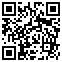
\includegraphics[width=0.25\textwidth]{prime_strings.png}
            \caption{\url{https://dlnnlsn.github.io/prime-strings}}
        \end{figure}
    \end{itemize}

\end{frame}

\end{document}